
\section{Dataset}
This section introduces how we build the whole dataset from raw data.

TODO: 这里插一张总体流程图

\subsection{Data Description}
Our data is taken from the records of GPS devices on the taxis in Shenzhen. A brief description is as the following:
\begin{itemize}
    \item \textbf{Region:} Shenzhen
    \item \textbf{Time Range:} June 2020
    \item \textbf{Content:} Taxi GPS records
    \begin{itemize}
      \item License number
      \item Longitude and latitude
      \item Speed
      \item Timestamp
    \end{itemize}
  \item \textbf{Size:} Over 2,700,000,000 rows
\end{itemize}

A small part of data is shown as an example in figure \ref{fig: raw_data}.
\begin{figure}[htb]
    \centering
    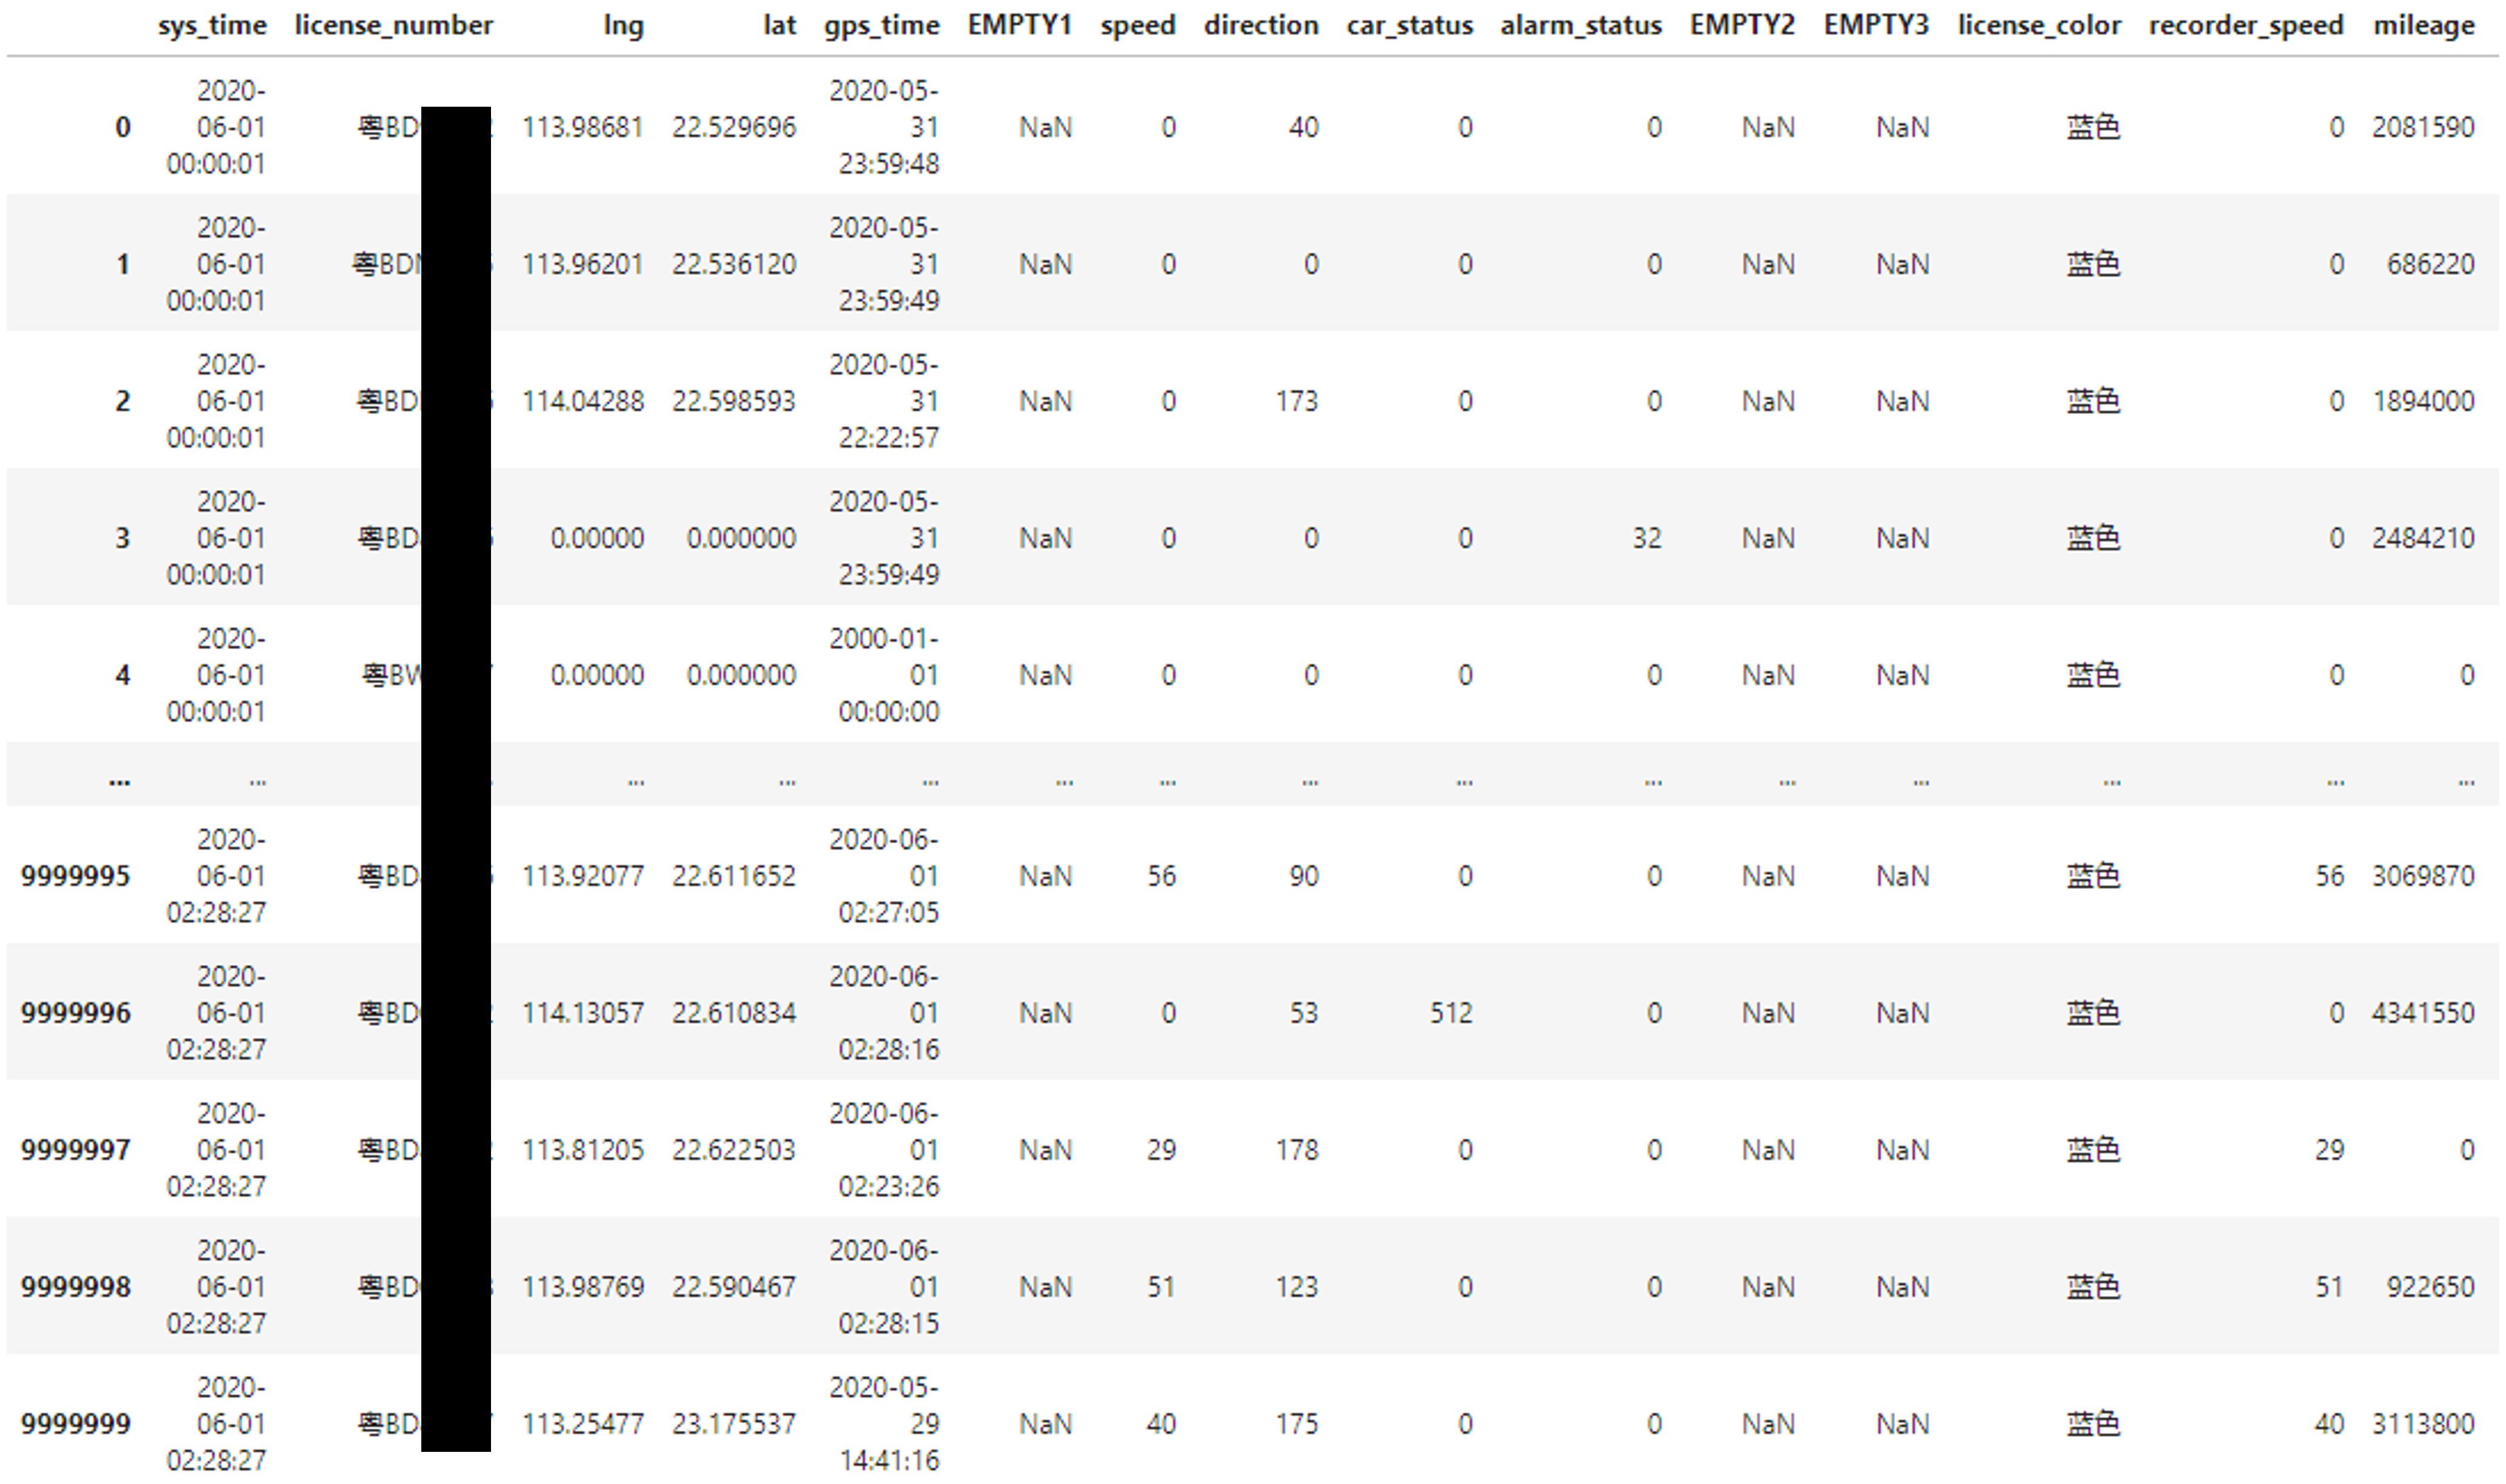
\includegraphics[width=\textwidth]{images/raw_data.png}
    \caption{Shenzhen taxi GPS raw data}
    \label{fig: raw_data}
\end{figure}

Unlike the open datasets that can be applied to deep learning models without the need of data cleaning and completion, this raw dataset contains lots of abnormal values, which should be cleaned and re-organized carefully.

\subsection{Data Cleaning}
Data cleaning is the process of detecting and correcting (or removing) corrupt or inaccurate records from a record set, table, or database and refers to identifying incomplete, incorrect, inaccurate or irrelevant parts of the data and then replacing, modifying, or deleting the dirty or coarse data\cite{data_cleaning}. There are many kinds of bad records that should be deleted or modified. To summarize, we categorize them as the following classes.

\begin{enumerate}
  \item \textbf{Duplicate Rows}. A considerable large part of the raw data are duplicate. The reason is when a GPS device is transmitting data to server, it will send several copies in order to avoid packet loss under poor Internet connection. As a result, they are completely same rows, and thus can be removed safely, leaving only the foremost one.
  \item \textbf{Corrupted Timestamp}.
\end{enumerate}
